\documentclass[12pt,3p]{article}
\usepackage[utf8]{inputenc}
\usepackage[english]{babel}
 \usepackage[margin=0.5in]{geometry}
 \usepackage{amsmath}
 \usepackage{amssymb}
\usepackage{mathtools}
\usepackage{enumitem}
\usepackage{physics}
% For different colored text 
\usepackage{xcolor}
\usepackage[round,numbers]{natbib}
\usepackage[colorlinks = false]{hyperref}
\usepackage{graphicx}
\usepackage{subcaption}

\numberwithin{equation}{section}

\begin{document}

%====================================================================================
%====================================================================================
%====================================================================================
%====================================================================================
\title{Personal Notes on Paper: \\
	\large{Gradient Damage Models and Their Use to Approximate Brittle Fracture}}
\author{Kim Pham, Hanen Amor, Jean-Jacques Marigo and Carrado Maurini}
\date{\vspace{-5ex}}
\maketitle

\tableofcontents
\newpage

\section{Definitions}
%====================================================================================
%====================================================================================
%====================================================================================
$\alpha$: Damage variable growing from 0 (undamaged) to 1 (damaged) [Dimensionless] \\
$\nabla \alpha (x)$: local gradient of the damage field at x where $\nabla \alpha(x) = 0$ indicates a homogenous damage process 
\begin{equation*}
\bigg[ \frac{1}{\text{Length}} \bigg] 
\end{equation*}
$W_l$: state function which gives the energy density at each point x 
\begin{equation*}
\bigg[ \frac{\text{Energy}}{\text{Volume}} = \frac{N \cdot m}{m^3} = \frac{N}{m^2} \bigg]
\end{equation*}
l: material characteristic length that controls the thickness of the damage localization zone \\
$w_1 = w(1)$: Specific fracture energy of the brittle damage material 
\begin{equation*}
\bigg[ \frac{\text{Energy}}{\text{Volume}} = \frac{N \cdot m}{m^3} = \frac{N}{m^2} \bigg]
\end{equation*}
$w(\alpha)$: Density of the energy dissipated by the material during a homogeneous damage process 
\begin{equation*}
\bigg[ \frac{\text{Energy}}{\text{Volume}} = \frac{N \cdot m}{m^3} = \frac{N}{m^2} \bigg]
\end{equation*}
$A(\alpha)$: Rigidity of the material in the damage state $\alpha$, or stiffness function
\begin{equation*}
\bigg[ \frac{\text{Energy}}{\text{Volume}} = \frac{N \cdot m}{m^3} = \frac{N}{m^2} \bigg]
\end{equation*}
 $S(\alpha) = A^{-1} (\alpha)$: Compliance function \\
$\textbf{u}$: Displacement [m] \\
$\boldsymbol{\varepsilon} (\mathbf{u})$: local linearized strain [Dimensionless] \\ \\
% ------
$H^{1} (\Omega)$: Sobolev space of functions defined on $\Omega$ which are square integrable and have square integrable first derivatives \\
$\mathbf{U_t}$: Imposed displacement on the boundary part $\partial \Omega_U$ \\
$\mathbf{F_t}$: Surface forces on the complementary boundary part $\partial \Omega_F$ [$\frac{N}{m^2}$]  \\
$\mathbf{f_t}$: Volume (body) forces over the domain $\Omega$ [$\frac{N}{m^2}$] \\
$\mathcal{P}_t (\mathbf{u}, \alpha) $: Total energy [Energy = $N \cdot m$] \\
$\mathcal{E} (\mathbf{u}, t)$: Total strain energy \\ \\
% ------
$\mathcal{D}$: convex cone of positive damage rate \\
$\mathcal{D} \mathcal{P}_t (\mathbf{u}, \alpha) (\mathbf{v}, \beta)$: Gateaux derivative of the total energy at ($ \mathbf{u}, \alpha$) and ($\mathbf{v}, \beta$) \\
$\boldsymbol{\sigma}_{t}$: stress at time t [$\frac{N}{m^2}$] \\ \\
% ------
\(\mathcal{H}^{n-1}\): Surface measure of $\Gamma$ \\
$G_c$: material toughness, the energy required to create a unit crack surface according to Griffith's Theory
\begin{equation*}
\bigg[ \frac{\text{Energy}}{\text{Area}} = \frac{N \cdot m }{m^2} = \frac{N}{m} \bigg] 
\end{equation*} \\
% ------
$U_t$: Displacement at time t [Length = m] \\
$U_e$: Displacement at elastic limit \\
$\sigma_e$: Stress at elastic limit \\
$\sigma_m$: maximum or peak stress that the material can sustain

\newpage
%==========================================================================
%==========================================================================
%==========================================================================
\section{Variational Formulation of Isotropic Damage Models}
%==========================================================================
%==========================================================================
\subsection{Constitutive Assumptions}
We can assume that the state function of energy density takes the following form:
\begin{align}\label{EnergyDensity}
\begin{split}
W_l (\boldsymbol{\varepsilon} (\mathbf{u}), \alpha, \nabla \alpha) &= \underbrace{ \frac{1}{2} A (\alpha) \boldsymbol{\varepsilon} (\mathbf{u}) \cdot \boldsymbol{\varepsilon} (\mathbf{u})}_\text{Elastic energy} + \underbrace{w (\alpha)}_\text{Homogeneous damage process} + \underbrace{\frac{1}{2} w_l l^2 \nabla \alpha \cdot \nabla \alpha}_\text{Nonlocal contribution}	
\end{split}
\end{align}
The last term in particularly plays a regularizing role by limiting the possibilities of localization of the damage field. In other words, the term, $1/2 w_1 l^2$, acts as a penalty on the gradient of $\alpha$, holding the profile fixed to a certain width. See Fig 5. from the paper. 
%-----------------------------------------------------------------------------------------------------------------------------------
\begin{figure}[h]
    \centering
    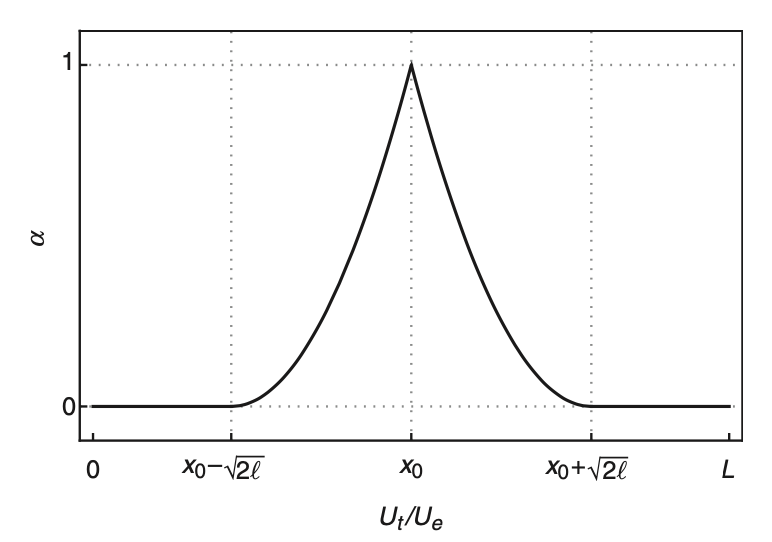
\includegraphics[width=0.5\textwidth]{Images/Fig5.png}
    \caption{Example of profile limited by the material characteristic length, l}
\end{figure}

The qualitative properties of the damage model depend on properties of the stiffness function, $A(\alpha)$, the dissipation function, $w(\alpha)$, the compliance function, $S(\alpha) = A^{-1} (\alpha)$, and their derivatives. These three functions must be continuously differentiable on $\alpha = [0, 1]$ and fulfill the following conditions: 
\begin{align}\label{Hypothesis1}
\begin{split}
\text{Positive elasticity}:& \quad A(\alpha) > 0, \, S(\alpha) > 0 \quad \text{with } A(1) = 0 \\
\text{Decreasing Stiffness}:& \quad A'(\alpha) < 0, \, S'(\alpha) > 0 \\
\text{Dissipation}:& \quad w(0) = 0, \, w(\alpha \neq 0) > 0, w'(\alpha) \geq 0
\end{split}
\end{align}
In the first condition $A(1) = 0$ says that when the material is damaged, the elasticity is zero. In the second condition, we can recall that the compliance function is related to the inverse of the dissipation function. The last condition states that when the material is undamaged, there is no dissipation, but when the material damages, some energy is dissipated. Furthermore, the derivative of the dissipation function must be positive, because energy cannot return into the material system. 

%==========================================================================
%==========================================================================
\subsection{Energy Functional}
Define the space of kinematically admissible displacement fields at time t as: 
\begin{equation}\label{KinDispFields}
\mathcal{C}\left(\mathbf{U}_{t}\right)=\left\{\mathbf{v} \in\left(H^{1}(\Omega)\right)^{n}: \mathbf{v}=\mathbf{U}_{t} \text { on } \partial_{U} \Omega\right\}
\end{equation}
where $H^{1} (\Omega)$ are the Sobolev space of functions defined on the domain which are square integrable and have square integrable first derivatives. \\ \\
Define the space of kinetically admissible damage fields in the subset $\beta$ of the Sobolev space $H^{1} (\Omega)$
\begin{equation}\label{KinDamFields}
\mathcal{D}_{1}=\left\{\beta \in H^{1}(\Omega): \beta(x) \in[0,1] \text { for almost all } x\right\}
\end{equation}
Define the total energy using the definition for Eq. \ref{EnergyDensity}.
\begin{align}\label{TotalEnergy}
\begin{split}
\mathcal{P}_t (\mathbf{u}, \alpha) &= \mathcal{E} (\mathbf{u}, ) - \int_{\Omega} \mathbf{f_t} \cdot \mathbf{u} d \Omega \int_{\partial_F \Omega} - \mathbf{F_t} \cdot \mathbf{u} d \Gamma \\
						   &= \int_{\Omega} W_l (\boldsymbol{\varepsilon} (\mathbf{u}), \alpha (x), \nabla \alpha (x)) d \Omega - \int_{\Omega} \mathbf{f_t} \cdot \mathbf{u} d \Omega - \int_{\partial_F \Omega} \mathbf{F_t} \cdot \mathbf{u} d \Gamma \\
						   &= \int_{\Omega} \bigg[ \frac{1}{2} A (\alpha) \boldsymbol{\varepsilon} (\mathbf{u}) \cdot \boldsymbol{\varepsilon} (\mathbf{u}) + w (\alpha) + \frac{1}{2} w_1 l^2 \nabla \alpha \cdot \nabla \alpha \bigg] d \Omega - \int_{\Omega} \mathbf{f_t} \cdot \mathbf{u} d \Omega - \int_{\partial_F \Omega} \mathbf{F_t} \cdot \mathbf{u} d \Gamma \\
\mathcal{P}_t (\mathbf{u}, \alpha) &= \int_{\Omega} \frac{1}{2} A (\alpha) \boldsymbol{\varepsilon} (\mathbf{u}) \cdot \boldsymbol{\varepsilon} (\mathbf{u}) d \Omega + \int_{\Omega} w (\alpha) d \Omega + \int_{\Omega} \frac{1}{2} w_1 l^2 \nabla \alpha \cdot \nabla \alpha d \Omega - \int_{\Omega} \mathbf{f_t} \cdot \mathbf{u} d \Omega - \int_{\partial_F \Omega} \mathbf{F_t} \cdot \mathbf{u} d \Gamma
\end{split}
\end{align}
where the total strain energy is defined as: 
\begin{align}\label{TotalStrainEnergy}
\mathcal{E} (\mathbf{u}, t)  = \int_{\Omega} W_l (\boldsymbol{\varepsilon} (\mathbf{u}), \alpha (x), \nabla \alpha (x)) d \Omega
\end{align}

%==========================================================================
%==========================================================================
\subsection{First-order Optimality Conditions: Evolution, Eq'm, and Damage}
The following variational evolution problem is stated below: \\
For each t $>$ 0, find $(\mathbf{u}_t, \alpha_t)$ in $\mathcal{C} (\mathbf{U}_t) \times \mathcal{D}_1$ such that 
\begin{align}\label{statementVarProblem}
\begin{split}
(\dot{\mathbf{u}}_t, \dot{\alpha}_t) \in \mathcal{C} (\dot{\mathbf{U}}_t) \times \mathcal{D} \quad \text{and} \quad \forall (\mathbf{v}, \beta) \in \mathcal{C} (\dot{\mathbf{U}}_t) \times \mathcal{D}, \\
D \mathcal{P} (\mathbf{u}_t, \alpha_t) (\mathbf{v} - \dot{\mathbf{u}}_t, \beta - \dot{\alpha}_t) \geq 0
\end{split}
\end{align} 
where $\mathcal{D}$ denotes the convex cone of positive damage rate:
\begin{equation*}
\mathcal{D} = \big\{ \beta \in H^1 (\Omega) : \beta(x) \geq 0 \quad \text{for almost all x} \big\} 
\end{equation*}
We can calculate the variations separately referring to the appendix (Appendix \ref{App:Gateaux}), to determine how to calculate the Gateaux derivative. The essential idea is the minimization can be done piecewise and added together to obtain the full minimization. 
\begin{align}\label{PartGateaux}
\begin{split}
\mathcal{D} \mathcal{P} (\mathbf{u}, \alpha) (\mathbf{v}, \beta) = \frac{d}{d \delta} P_t (\mathbf{u} + \delta \mathbf{v}, \alpha + \delta \beta) \bigg\rvert_{\delta = 0} = \frac{d}{d \delta} P_t (\mathbf{u}+ \delta \mathbf{v}, \alpha) \bigg\rvert_{\delta = 0} + \frac{d}{d \delta} P_t (\mathbf{u}, \alpha + \delta \beta) \bigg\rvert_{\delta = 0}
\end{split}
\end{align}
Piecewise, we can first evaluate the first term of Eq. \ref{PartGateaux}. 
\begin{align*}
\begin{split}
P_t (\mathbf{u}+ \delta \mathbf{v}, \alpha) = \int_{\Omega} W_l (\boldsymbol{\varepsilon}(\mathbf{u} + \delta \mathbf{v}), \alpha, \nabla \alpha) d \Omega
\end{split}
\end{align*}
Take the derivative, using the chain rule. See end of section for the calculations of each partial:
\begin{align*}
\begin{split}
\frac{d}{d \delta} P_t (\mathbf{u} + \delta \mathbf{v}, \alpha) 
&= \int_{\Omega} \frac{d}{d \delta} \bigg[ W_l (\boldsymbol{\varepsilon}(\mathbf{u} + \delta \mathbf{v}), \alpha, \nabla \alpha) \bigg] d \Omega \\
&= \int_{\Omega} \bigg[ \pdv{\boldsymbol{\varepsilon} (\mathbf{u} + \delta \mathbf{v})}{\delta} \pdv{W_l \big( \boldsymbol{\varepsilon}(\mathbf{u} + \delta \mathbf{v}), \alpha, \nabla \alpha \big) }{\boldsymbol{\varepsilon} (\mathbf{u} + \delta \mathbf{v})} \bigg] d \Omega \\
&= \int_{\Omega} \big[ \mathbf{v} \boldsymbol{\varepsilon} (\mathbf{u} + \delta \mathbf{v}) \cdot A(\alpha) \boldsymbol{\varepsilon} (\mathbf{u} + \delta \mathbf{v}) \big] d \Omega \\
\frac{d}{d \delta} P_t (\mathbf{u} + \delta \mathbf{v}, \alpha) &= \int_{\Omega} \mathbf{v} A(\alpha) \boldsymbol{\varepsilon} (\mathbf{u} + \delta \mathbf{v}) \cdot \boldsymbol{\varepsilon} (\mathbf{u} + \delta \mathbf{v}) d \Omega 
\end{split}
\end{align*}
Evaluate as $\delta = 0$
\begin{align*}
\frac{d}{d \delta} P_t (\mathbf{u} + \delta \mathbf{v}, \alpha) \bigg\rvert_{\delta = 0} = \int_{\Omega} \mathbf{v} A(\alpha) \boldsymbol{\varepsilon} (\mathbf{u}) \cdot \boldsymbol{\varepsilon} (\mathbf{u}) d \Omega
\end{align*}
Next, we can evaluate the second term of Eq. \ref{PartGateaux}. Note that we assume that $\nabla (\alpha + \delta \beta) = \nabla \alpha + \delta \nabla \beta$. 
\begin{align*}
P_t (\mathbf{u}, \alpha + \delta \beta) = \int_{\Omega} W_l (\boldsymbol{\varepsilon}(\mathbf{u}, \alpha + \delta \beta, \nabla \alpha + \delta \nabla \beta) d \Omega
\end{align*}
Take the derivative using the chain rule. See end of section for the calculation of each partial. 
\begin{align*}
\frac{d}{d \delta} P_t (\mathbf{u}, \alpha + \delta \beta) &= \int_{\Omega} \frac{d}{d \delta} W_l (\boldsymbol{\varepsilon}(\mathbf{u}, \alpha + \delta \beta, \nabla \alpha + \delta \nabla \beta) d \Omega \\
        &= \int_{\Omega} \bigg[ \pdv{(\alpha + \delta \beta)}{\delta} \pdv{W_l}{(\alpha + \delta \beta)} + \pdv{(\nabla \alpha + \delta \nabla \beta)}{\delta} \pdv{W_l}{(\nabla \alpha + \delta \nabla \beta)} \bigg] d \Omega \\
        &= \int_{\Omega} \bigg[ \beta \pdv{W_l}{(\alpha + \delta \beta)} +\nabla \beta \pdv{W_l}{(\nabla \alpha + \delta \nabla \beta)} \bigg] d \Omega \\
\frac{d}{d \delta} P_t (\mathbf{u}, \alpha + \delta \beta) &= \int_{\Omega} \bigg[ \beta \big[ \frac{1}{2} A'(\alpha + \delta \beta) \boldsymbol{\varepsilon} (\mathbf{u}) \cdot \boldsymbol{\varepsilon} (\mathbf{u}) + w'(\alpha + \delta \beta) \big] + \nabla \beta \cdot \big[ w_1 l^2 (\nabla \alpha + \delta \nabla \beta) \big] \bigg] d \Omega  
\end{align*}
Evaluate as $\delta = 0$:
\begin{align*}
\frac{d}{d \delta} P_t (\mathbf{u}, \alpha + \delta \beta) \bigg\rvert_{\delta = 0} &= \int_{\Omega} \bigg[ \beta \big[ \frac{1}{2} A'(\alpha) \boldsymbol{\varepsilon} (\mathbf{u}) \cdot \boldsymbol{\varepsilon} (\mathbf{u}) + w'(\alpha) \big] + \nabla \beta \cdot \big[ w_1 l^2 (\nabla \alpha ) \big] \bigg] d \Omega \\
\frac{d}{d \delta} P_t (\mathbf{u}, \alpha + \delta \beta) \bigg\rvert_{\delta = 0} &= \int_{\Omega} \beta \bigg[ \frac{1}{2} A'(\alpha) \boldsymbol{\varepsilon} (\mathbf{u}) \cdot \boldsymbol{\varepsilon} (\mathbf{u}) + w'(\alpha) \bigg] d \Omega + \int_{\Omega} w_1 l^2 \nabla \alpha \cdot \nabla \beta d \Omega
\end{align*}
Combining each part into one equation (Eq. \ref{PartGateaux}) gives, 
\begin{align*}
\begin{split}
\frac{d}{d \delta} P_t (\mathbf{u}+ \delta \mathbf{v}, \alpha + \delta \beta) \bigg\rvert_{\delta = 0} &= \frac{d}{d \delta} P_t (\mathbf{u}+ \delta \mathbf{v}, \alpha) \bigg\rvert_{\delta = 0} + \frac{d}{d \delta} P_t (\mathbf{u}, \alpha + \delta \beta) \bigg\rvert_{\delta = 0} \\
&= \int_{\Omega} \mathbf{v} A(\alpha) \boldsymbol{\varepsilon} (\mathbf{u}) \cdot \boldsymbol{\varepsilon} (\mathbf{u}) d \Omega \\
        &+ \int_{\Omega} \beta \bigg[ \frac{1}{2} A'(\alpha) \boldsymbol{\varepsilon} (\mathbf{u}) \cdot \boldsymbol{\varepsilon} (\mathbf{u}) + w'(\alpha) \bigg] d \Omega + \int_{\Omega} w_1 l^2 \nabla \alpha \cdot \nabla \beta d \Omega
\end{split}
\end{align*}
Leaving the result for the Gateaux derivative of $\mathcal{P}$ at $(\mathbf{u}, \alpha)$ in the direction of $(\mathbf{v}, \beta)$
\begin{align}\label{Gateaux}
\mathcal{D} \mathcal{P} (\mathbf{u}, \alpha) (\mathbf{v}, \beta) = \int_{\Omega} \mathbf{v} A(\alpha) \boldsymbol{\varepsilon} (\mathbf{u}) \cdot \boldsymbol{\varepsilon} (\mathbf{u}) d \Omega + \int_{\Omega} \beta \bigg[ \frac{1}{2} A'(\alpha) \boldsymbol{\varepsilon} (\mathbf{u}) \cdot \boldsymbol{\varepsilon} (\mathbf{u}) + w'(\alpha) \bigg] d \Omega + \int_{\Omega} w_1 l^2 \nabla \alpha \cdot \nabla \beta d \Omega
\end{align}
\textcolor{red}{Note that we have an extra $\mathbf{v}$ in the first integral as compared to Equation 9 in the paper.} This might be because $A(\alpha) \boldsymbol{\varepsilon} (\mathbf{u}) \cdot \boldsymbol{\varepsilon} (\mathbf{u})$ holds for any kinematically admissible test function $\mathbf{v}$ 

%===================================================================================
\subsubsection{Proof of Equations 10 and 11}
If we utilize integration by parts on the last term, we can quickly note that Eq. \ref{Gateaux} holds for all variations, $\mathbf{v}$ or $\beta$, and the first integral lead to the standard equilibrium equation and the remaining integrals lead to the Karush-Kuhn-Tucker (KKT) conditions. \\ \\
The equilibrium equation can be obtained by recognizing $\boldsymbol{\sigma} = A(\alpha) \boldsymbol{\varepsilon} (\mathbf{u})$
\begin{align*}
\int_{\Omega} \mathbf{v} A(\alpha) \boldsymbol{\varepsilon} (\mathbf{u}) \cdot \boldsymbol{\varepsilon} (\mathbf{u}) d \Omega &= 0 \\ 
\int_{\Omega} \mathbf{v} ( \boldsymbol{\sigma} \cdot \boldsymbol{\varepsilon} (\mathbf{u})) d \Omega &= 0 \\
\int_{\Omega} \boldsymbol{\sigma} \cdot \boldsymbol{\varepsilon} (\mathbf{u}) d \Omega &= 0 
\end{align*}
where we can recognize that strain $\boldsymbol{\varepsilon} (\mathbf{u}) = \partial \mathbf{u} / \partial x$. Therefore, we can do integration by parts, where $\mathbf{u}$ is displacement. 
\begin{align*}
\pdv{}{x_j} \big( \sigma_{ij} u_i \big) &= \pdv{\sigma_{ij}}{x_j} u_i + \sigma_{ij} \pdv{u_i}{x_j} \\
\pdv{}{x_j} \big( \sigma_{ij} u_i \big) - \pdv{\sigma_{ij}}{x_j} u_i &= \sigma_{ij} \pdv{u_i}{x_j} \\
\pdv{}{x} \big( \boldsymbol{\sigma} \cdot \mathbf{u} \big) - \pdv{\boldsymbol{\sigma}}{x} \cdot \mathbf{u} &= \boldsymbol{\sigma} \cdot \pdv{\mathbf{u}}{x}
\end{align*}
Substituting back 
\begin{align*}
\int_{\Omega} \boldsymbol{\sigma} \cdot \boldsymbol{\varepsilon} (\mathbf{u}) d \Omega = \int_{\Omega} \boldsymbol{\sigma} \cdot \pdv{\mathbf{u}}{x} d \Omega 
&= \int_{\Omega} \pdv{}{x} \big( \boldsymbol{\sigma} \cdot \mathbf{u} \big) d \Omega - \int_{\Omega} \pdv{\boldsymbol{\sigma}}{x} \cdot  \mathbf{u} = 0 \quad \text{Divergence} \\
&= \int_{\Gamma} ( \boldsymbol{\sigma} \mathbf{n} ) \cdot \mathbf{u} d \Gamma - \int_{\Omega} \pdv{\boldsymbol{\sigma}}{x} \cdot \mathbf{u} d \Omega = 0 
\end{align*}
This holds for all $\mathbf{u}$; therefore we can obtain two important expressions, including the equilibrium expression
\begin{equation}
\pdv{\boldsymbol{\sigma}}{x} + \mathbf{f_t} = 0 \quad \text{and} \quad \boldsymbol{\sigma_t} \mathbf{n} = \mathbf{F_t}
\end{equation}
Next, we can do integration by parts for the last term of Eq. \ref{Gateaux}:
\begin{align*}
(f'g)'&= f''g + f' g' \\
\pdv[2]{\alpha}{x_i} \beta &= \bigg( \pdv{\alpha}{x_i} \beta \bigg)_{,i} + \pdv{\alpha}{x_i} \pdv{\beta}{x_j} \\
\beta \nabla^2 \alpha &= \frac{d}{dx} (\nabla \alpha \cdot \beta)+ \nabla \alpha \cdot \nabla \beta \\
\beta \nabla^2 \alpha - \frac{d}{dx} (\nabla \alpha \cdot \beta) &= \nabla \alpha \cdot \nabla \beta 
\end{align*}
Substitute into the last part of equation \ref{Gateaux} related to the variation in the direction of $\beta$. We can achieve the following form. 
\begin{align*}
\int_{\Omega} \beta \bigg[ \frac{1}{2} A'(\alpha) \boldsymbol{\varepsilon} (\mathbf{u}) \cdot \boldsymbol{\varepsilon} (\mathbf{u}) + w'(\alpha) \bigg] d \Omega + \int_{\Omega} w_1 l^2 \nabla \alpha \cdot \nabla \beta d \Omega &= 0 \\
\int_{\Omega} \beta \bigg[ \frac{1}{2} A'(\alpha) \boldsymbol{\varepsilon} (\mathbf{u}) \cdot \boldsymbol{\varepsilon} (\mathbf{u}) + w'(\alpha) \bigg] d \Omega + \int_{\Omega} w_1 l^2 \bigg[ \beta \nabla^2 \alpha - \frac{d}{dx} (\nabla \alpha \cdot \beta) \bigg] d \Omega &= 0 \quad \text{Rearrange} \\ 
\int_{\Omega} \beta \bigg[ \frac{1}{2} A'(\alpha) \boldsymbol{\varepsilon} (\mathbf{u}) \cdot \boldsymbol{\varepsilon} (\mathbf{u}) + w'(\alpha) + w_1 l^2 \nabla^2 \alpha \bigg] d \Omega - \int_{\Omega} w_1 l^2 \frac{d}{dx} (\nabla \alpha \cdot \beta) d \Omega &= 0 \quad \text{Divergence} \\
\int_{\Omega} \beta \bigg[ \frac{1}{2} A'(\alpha) \boldsymbol{\varepsilon} (\mathbf{u}) \cdot \boldsymbol{\varepsilon} (\mathbf{u}) + w'(\alpha) + w_1 l^2 \nabla^2 \alpha \bigg] d \Omega - \int_{\Gamma} w_1 l^2 \nabla \alpha \mathbf{n} \cdot \beta d \Gamma &= 0 \\
\int_{\Omega} \beta \bigg[ \frac{1}{2} A'(\alpha) \boldsymbol{\varepsilon} (\mathbf{u}) \cdot \boldsymbol{\varepsilon} (\mathbf{u}) + w'(\alpha) + w_1 l^2 \nabla^2 \alpha \bigg] d \Omega &= 0 
\end{align*}
where we have assumed the boundary term goes to zero by \textcolor{red}{$\pdv{\alpha}{x} \mathbf{n} = \pdv{\alpha}{n} = 0$} \\ \\ 
From this equation, we have derived the strong form for the damage evolution problem in the form of the KKT conditions for unilateral constrained variational problems where $\beta = \dot{\alpha}_t$: 
\begin{align}\label{kktCond}
\begin{split}
\text{Irreversibility: }&
\dot{\alpha}_t \geq 0 \quad \text{on } \Omega \\
\text{Damage criterion: }&
\frac{1}{2} A'(\alpha) \boldsymbol{\varepsilon} (\mathbf{u}) \cdot \boldsymbol{\varepsilon} (\mathbf{u}) + w'(\alpha) - w_1 l^2 \nabla^2 \alpha \geq 0 \quad \text{on } \Omega \\
\text{Energy Balance: }&
\dot{\alpha}_t \bigg[ \frac{1}{2} A'(\alpha) \boldsymbol{\varepsilon} (\mathbf{u}) \cdot \boldsymbol{\varepsilon} (\mathbf{u}) + w'(\alpha) - w_1 l^2 \nabla^2 \alpha \bigg] = 0  \quad \text{on } \Omega
\end{split}
\end{align}
The first statement states that damage can only increase and the rate of damage must increase. The energy balance states that if the damage criterion is an equality (= 0), then the damage can only increase.  

%===================================================================================
\subsubsection{Calculations for the partials} 
Calculate the first partial of the first term in Eq. \ref{PartGateaux}. 
\begin{align*}
\begin{split}
\pdv{\boldsymbol{\varepsilon} (\mathbf{u} + \delta \mathbf{v})}{\delta} &= \mathbf{v} \boldsymbol{\varepsilon} (\mathbf{u} + \delta \mathbf{v})
\end{split}
\end{align*}
Rewrite Eq. \ref{EnergyDensity} and calculate the second partial: 
\begin{align*}
\begin{split}
W_l (\boldsymbol{\varepsilon} (\mathbf{u} + \delta \mathbf{v}), \alpha, \nabla \alpha) &= \frac{1}{2} A (\alpha) \boldsymbol{\varepsilon} ((\mathbf{u} + \delta \mathbf{v})) \cdot \boldsymbol{\varepsilon} ((\mathbf{u} + \delta \mathbf{v})) + w (\alpha) + \frac{1}{2} w_l l^2 \nabla \alpha \cdot \nabla \alpha	\\
\frac{d W_l}{d \boldsymbol{\varepsilon} (\mathbf{u} + \delta \mathbf{v})} &= \frac{1}{2} A(\alpha) \bigg[ \frac{d \boldsymbol{\varepsilon} (\mathbf{u} + \delta \mathbf{v})}{d \boldsymbol{\varepsilon} (\mathbf{u} + \delta \mathbf{v})} \cdot \boldsymbol{\varepsilon} (\mathbf{u} + \delta \mathbf{v}) + \boldsymbol{\varepsilon} (\mathbf{u} + \delta \mathbf{v}) \cdot \frac{d \boldsymbol{\varepsilon} (\mathbf{u} + \delta \mathbf{v})}{d \boldsymbol{\varepsilon} (\mathbf{u} + \delta \mathbf{v})} \bigg] \\
        &= \frac{1}{2} A(\alpha) \big[ \boldsymbol{\varepsilon} (\mathbf{u} + \delta \mathbf{v}) + \boldsymbol{\varepsilon} (\mathbf{u} + \delta \mathbf{v}) \big] \\
\frac{d W_l}{d \boldsymbol{\varepsilon} (\mathbf{u} + \delta \mathbf{v})} &= A(\alpha) \boldsymbol{\varepsilon} (\mathbf{u} + \delta \mathbf{v})
\end{split}
\end{align*}
Calculate the first partial for the second part of  Eq. \ref{PartGateaux} by rewriting Eq. \ref{EnergyDensity}. 
\begin{align*}
\begin{split}
W_l (\boldsymbol{\varepsilon} (\mathbf{u}), \alpha + \delta \beta , \nabla \alpha + \delta \nabla \beta) &= \frac{1}{2} A (\alpha + \delta \beta) \boldsymbol{\varepsilon} (\mathbf{u}) \cdot \boldsymbol{\varepsilon} (\mathbf{u}) + w (\alpha + \delta \beta) + \frac{1}{2} w_l l^2 ( \nabla \alpha + \delta \nabla \beta) \cdot (\nabla \alpha + \delta \nabla \beta) \\
\end{split}
\end{align*}
Calculations: 
\begin{align*}
\pdv{W_l}{(\alpha + \delta \beta)} &= \frac{1}{2} A'(\alpha + \delta \beta) \boldsymbol{\varepsilon} (\mathbf{u}) \cdot \boldsymbol{\varepsilon} (\mathbf{u}) + w'(\alpha + \delta \beta)
\end{align*}
\begin{align*}
\pdv{W_l}{(\nabla \alpha + \delta \nabla \beta)} &= \frac{1}{2} w_1 l^2 \bigg[ \pdv{(\nabla \alpha + \delta \nabla \beta)}{(\nabla \alpha + \delta \nabla \beta)} \cdot (\nabla \alpha + \delta \nabla \beta) + (\nabla \alpha + \delta \nabla \beta) \cdot \pdv{(\nabla \alpha + \delta \nabla \beta)}{(\nabla \alpha + \delta \nabla \beta)} \bigg] \\
                &= \frac{1}{2} w_1 l^2 \big[(\nabla \alpha + \delta \nabla \beta) + (\nabla \alpha + \delta \nabla \beta) \big] \\
\pdv{W_l}{(\nabla \alpha + \delta \nabla \beta)} &= w_1 l^2 (\nabla \alpha + \delta \nabla \beta)
\end{align*}

%===================================================================================
%===================================================================================
\subsection{Strain Hardening and Stress Softening}
A material is said to be strain hardening when \(\alpha \mapsto\left(-A^{\prime}(\alpha) / w^{\prime}(\alpha)\right)\) is decreasing with respect to $\alpha$:
\begin{align}\label{strainHardening}
w^{\prime}(\alpha) \mathrm{A}^{\prime \prime}(\alpha)-w^{\prime \prime}(\alpha) \mathrm{A}^{\prime}(\alpha)>0
\end{align}
The material is said to be stress hardening/softening when \(\alpha \mapsto\left(\mathbf{S}^{\prime}(\alpha) / w^{\prime}(\alpha)\right)\) is decreasing/increasing with respect to $\alpha$: 
\begin{align}\label{stressHardening}
\begin{split}
\text{Stress Hardening: }& w^{\prime}(\alpha) S^{\prime \prime}(\alpha)-w^{\prime \prime}(\alpha) S^{\prime}(\alpha) < 0 \\
\text{Stress Softening: }& w^{\prime}(\alpha) S^{\prime \prime}(\alpha)-w^{\prime \prime}(\alpha) S^{\prime}(\alpha) > 0
\end{split}
\end{align}
\textcolor{red}{Something familiar about the statement of these criterion. Mathematically convex?}

%===================================================================================
%===================================================================================
\subsection{Approximation of Variational Brittle Fracture}
The variational approach to brittle fracture formulates this evolution problem as a global minimization condition on the following Griffith energy functional, under an irreversibility condition for the crack set, $\Gamma$
\begin{align}\label{VarBrittleFracture}
\mathcal{F}(\mathbf{u}, \Gamma) 
&= \int_{\Omega \backslash \Gamma} \frac{1}{2} \mathbf{A}_{0} \varepsilon(\mathbf{u}) \cdot \varepsilon(\mathbf{u}) \mathrm{d} \Omega+G_{c} \mathcal{H}^{n-1}(\Gamma) \\
&= \int_{\Omega \backslash \Gamma} \frac{1}{2} \mathbf{A}_{0} \varepsilon(\mathbf{u}) \cdot \varepsilon(\mathbf{u}) \mathrm{d} \Omega + \int_{\Gamma} G_{c} \mathcal{H}^{n-1}(\Gamma) d \Gamma
\end{align}
Note that the first term is the elastic energy stored in the cracked body $\Omega \ \Gamma$ and the last term is the surface energy required to create the crack. In particular, $\mathcal{H}^{n-1}(\Gamma)$ is the surface measure of $\Gamma$. This expression is analogous to Eq. \ref{TotalStrainEnergy}
\begin{align}\label{SubTotalStrainEnergy}
\begin{split}
\mathcal{E} (\mathbf{u}, t) 
&= \int_{\Omega} W_l (\boldsymbol{\varepsilon} (\mathbf{u}), \alpha (x), \nabla \alpha (x)) d \Omega \\
&= \int_{\Omega} \frac{1}{2} A (\alpha) \boldsymbol{\varepsilon} (\mathbf{u}) \cdot \boldsymbol{\varepsilon} (\mathbf{u}) d \Omega + \int_{\Omega}  \big( w (\alpha) + \frac{1}{2} w_l l^2 \nabla \alpha \cdot \nabla \alpha \big) d \Omega
\end{split}
\end{align}
where the first term also indicates elastic energy, and the second the dissipative energy related to the crack ($w(\alpha)$ = dissipation function). Note that the main difference between Eq. \ref{VarBrittleFracture} and \ref{SubTotalStrainEnergy} is that the dissipative energy term is a surface integral in the Griffith energy functional and a volume integral in the damage model. \\ \\ 
Lastly, the equation for $G_c$, the material toughness is given as follows 
\begin{equation}\label{MatTough}
G_{c} = 2 \sqrt{2} \ell  \int_{0}^{1} \sqrt{w_{1} w(\beta)} \mathrm{d} \beta
\end{equation}

%===================================================================================
%===================================================================================
%===================================================================================
\section{Application to the 1D Tension Test}

%===================================================================================
%===================================================================================
\subsection{The 1D Problem}
The 1D bar of length, L, is made of a homogeneous material with stress softening. The end x = 0 is blocked while the end x = L has an imposed displacement, $U_t$. The admissible displacement field u must satisfy the boundary conditions (Eq. \ref{1DBC}) and no displacement is imposed in the initial time step. 
\begin{align}\label{1DBC}
u(x = 0) = 0, \quad u(x = L) = U_t = t L, \quad U_{t = 0} = 0
\end{align}
The total energy from Eq. \ref{TotalEnergy} assumes that there are no body and traction forces. 
\begin{align}\label{1DtotEnergy}
\begin{split}
\mathcal{P}_t (\mathbf{u}, \alpha) 
&= \int_{\Omega} \frac{1}{2} A (\alpha) \boldsymbol{\varepsilon} (\mathbf{u}) \cdot \boldsymbol{\varepsilon} (\mathbf{u}) d \Omega + \int_{\Omega} w (\alpha) d \Omega + \int_{\Omega} \frac{1}{2} w_1 l^2 \nabla \alpha \cdot \nabla \alpha d \Omega - \int_{\Omega} \mathbf{f_t} \cdot \mathbf{u} d \Omega - \int_{\partial_F \Omega} \mathbf{F_t} \cdot \mathbf{u} d \Gamma \\
\mathcal{P}_t (u, \alpha) 
&= \int_{\Omega} \frac{1}{2} E (\alpha) \boldsymbol{\varepsilon} (u) \cdot \boldsymbol{\varepsilon} (u) d \Omega + \int_{\Omega} w (\alpha) d \Omega + \int_{\Omega} \frac{1}{2} w_1 l^2 \nabla \alpha \cdot \nabla \alpha d \Omega
\end{split}
\end{align}
where $E(\alpha)$ is the 1D axial stiffness and $(.)' = \pdv{(.)}{x}$. The displacement is not a vector quantity and is denoted likewise. The 1D equilibrium equation is denoted as,
\begin{align}\label{1DEqm}
\begin{split}
\sigma_{t}^{\prime}(x) &= \pdv{\sigma_t}{x} = 0 \quad \text{no body force} \\
\sigma_{t}(x) = E\left(\alpha_{t}(x)\right) u_{t}^{\prime}(x) &= E \pdv{u}{x} = E \varepsilon, \quad \text{Hooke's Law}
\end{split}
\end{align}
The stress $\sigma_t$ along the bar is constant through the length, using Eq. \ref{1DEqm}
\begin{align}\label{1DStress}
\begin{split}
\sigma_t (x) &= E(\alpha_t(x)) \pdv{u_t}{x} \quad \text{Integrate over the length} \\
\int_0^L \sigma_t (x) &= \int_0^L E(\alpha_t(x)) \pdv{u_t}{x} dx \quad \text{Where the stress is constant through the length} \\
\sigma_t (x) &= \int_0^L E(\alpha_t(x)) dx \int_0^L \pdv{u_t}{x} dx \\
\sigma_t (x) &= \int_0^L E(\alpha_t(x)) dx \big[ u_t \big\rvert_L - u_t \big\rvert_0 \big] \quad \text{using boundary conditions in Eq. \ref{1DBC}} \\
\sigma_t (x) &= \int_0^L E(\alpha_t(x)) dx \big[ U_t - 0 \big] \quad \text{where } E(\alpha) = \frac{1}{S(\alpha)} \\
\sigma_t (x) &= \frac{U_t}{\int_0^L S(\alpha_t(x)) dx}
\end{split}
\end{align}
where the definition of S is $S(\alpha) = \frac{1}{E(\alpha)}$ \\ \\ 
Therefore the KKT conditions for the homogenous damage problem can be found from Eq. \ref{kktCond}. First we examine the irreversibility condition with an additional stipulation for no damage at time point 0. In other words, the bar is undamaged in the beginning of loading. 
\begin{align*}
\dot{\alpha}_t \geq 0 \quad \alpha_{0} = 0 
\end{align*}
The damage criterion can be modified with the knowledge that A is equivalent to E
\begin{align*}
\frac{1}{2} A'(\alpha) \boldsymbol{\varepsilon} (\mathbf{u}) \cdot \boldsymbol{\varepsilon} (\mathbf{u}) + w'(\alpha) - w_1 l^2 \nabla^2 \alpha &\geq 0 \\
\frac{1}{2} E'(\alpha_t) (u_t')^2 + w'(\alpha_t) - w_1 l^2 \alpha_t^{''} &\geq 0 
\end{align*}
The energy balance can also be rewritten
\begin{align*}
\dot{\alpha}_t \bigg[ \frac{1}{2} A'(\alpha) \boldsymbol{\varepsilon} (\mathbf{u}) \cdot \boldsymbol{\varepsilon} (\mathbf{u}) + w'(\alpha) - w_1 l^2 \nabla^2 \alpha \bigg] &= 0 \\
\dot{\alpha}_t \bigg[ \frac{1}{2} E'(\alpha_t) (u_t')^2 + w'(\alpha_t) - w_1 l^2 \alpha_t^{''} \bigg] &= 0 
\end{align*}
Therefore combining these three criterion, we achieve the KKT conditions 
\begin{align}\label{KKTCond1D}
\begin{split}
\text{Irreversibility: }&
\dot{\alpha}_t \geq 0 \quad \alpha_{0} = 0 \\
\text{Damage criterion: }&
\frac{1}{2} E'(\alpha_t) (u_t')^2 + w'(\alpha_t) - w_1 l^2 \alpha_t^{''} \geq 0 \\
\text{Energy Balance: }&
\dot{\alpha}_t \bigg[ \frac{1}{2} E'(\alpha_t) (u_t')^2 + w'(\alpha_t) - w_1 l^2 \alpha_t^{''} \bigg] = 0 
\end{split}
\end{align}
The boundary conditions are as follows: 
\begin{align}
\alpha_{t}^{\prime}(0) \leq 0, \quad \alpha_{t}^{\prime}(L) \geq 0
\end{align}
Lastly we note that there are at least two different length-scales to the problem. One is the length of the bar L, and the internal length, $l$. The uniqueness of the solution depends on the ratio between these lengthscales, $L/l$. 

%===================================================================================
%===================================================================================
\subsection{Homogeneous Solutions}
Homogeneous solutions are solutions for which the damage and the strain fields are uniform throughout the structure. The uniform strain field is stated as: 
\begin{align*}
\varepsilon = \pdv{u_t}{x} = u_t^{'} (x) = t \rightarrow u_t(x) = t x
\end{align*}
which we can then substitute into Hooke's law
\begin{align*}
\sigma_t = \varepsilon E = t E 
\end{align*}
For homogenous solutions eq. \ref{KKTCond1D}, $w_1 l^2 \nabla^2 \alpha_t$ term is zero because $\pdv{\alpha_t}{x}$ is zero. 
\begin{align*}
\begin{split}
\text{Irreversibility: }&
\dot{\alpha}_t \geq 0 \quad \alpha_{0} = 0 \\
\text{Damage criterion: }&
\frac{1}{2} E'(\alpha_t) (u_t')^2 + w'(\alpha_t) \geq 0 \\
\text{Energy Balance: }&
\dot{\alpha}_t \bigg[ \frac{1}{2} E'(\alpha_t) (u_t')^2 + w'(\alpha_t) \bigg] = 0 
\end{split}
\end{align*}
Therefore, using the statements for the uniform strain field, we have 
\begin{align}\label{KKTHomogSol}
\begin{split}
\frac{t^2}{2} E'(\alpha_t) + w'(\alpha_t) &\geq 0 \\
\dot{\alpha}_t \bigg[ \frac{t^2}{2} E'(\alpha_t) + w'(\alpha_t) \bigg] &= 0 
\end{split}
\end{align}

%===================================================================================
\subsubsection{Elastic Phase}
\textcolor{red}{Typo in equation for $\sigma_e$ in paper} \\ \\
\textcolor{blue}{Can expand the derivations in this section}
The elastic limit of displacement: 
\begin{equation}\label{elasticLimitDisp}
U_e = L \sqrt{- \frac{2 w'(0)}{E'(0)}}
\end{equation}
The yield stress
\begin{equation}\label{yieldStress}
\sigma_e = \sqrt{\frac{2w'(0)}{S'(0)}}
\end{equation}
The elastic phase is not observed if $w'(0) = 0$

%===================================================================================
\subsubsection{Damaging Phase}
\textcolor{blue}{Can expand the derivations in this section}
For $U_t \geq U_e$ the damage criterion becomes an equality and the damage can grow. Relationship between prescribed displacement, $U_t$ and the associated homogenous damage $\alpha_t$:
\begin{equation}\label{relDispDamage}
\frac{U_t}{L} = \sqrt{- \frac{2 w'(\alpha_t)}{E'(\alpha_T)}}
\end{equation}
Use equilibrium equation to give expression for stress, showing stress softening
\begin{equation}\label{stressTime}
\sigma_t = E(\alpha_t) t = \sqrt{\frac{2 w'(\alpha_t)}{S'(\alpha_t)}}
\end{equation}
Peak stress in homogenous solutions 
\begin{equation}\label{peakStress}
\sigma_M = \sup_{\alpha \in [0, 1]} \sqrt{\frac{2 w'(\alpha)}{S'(\alpha)}}
\end{equation}

\subsubsection{Example 1: A model with an Elastic Phase}
%====================================================================================
Consider the following damage law:
\begin{align}\label{ex1DamageLaw}
\begin{split}
E(\alpha) &= E_0 (1 - \alpha)^2 \rightarrow E'(\alpha) = - 2 E_0 (1 - \alpha)\\
w(\alpha) &= w_1 \alpha \rightarrow w'(\alpha) = w_1 
\end{split}
\end{align}
Note that the definition of S: 
\begin{align}\label{ex1S}
\begin{split}
S(\alpha) &= \frac{1}{E(\alpha)} \\
S(\alpha) &= \frac{1}{E_0 (1 - \alpha)^2} \rightarrow S'(\alpha) = \frac{2}{E_0 (1 - \alpha)^3}
\end{split}
\end{align}
Calculate the peak stress using Eq. \ref{peakStress}
\begin{align*}
\sigma_M &= \sup_{\alpha \in [0, 1]} \sqrt{\frac{2 w_1}{ \frac{2}{E_0 (1 - \alpha)^3} }} \\
		&= \sup_{\alpha \in [0, 1]} \sqrt{w_1 E_0 (1 - \alpha)^3} \quad \text{where the supremum value is where } \alpha = 0 \\
\sigma_M &= \sqrt{w_1 E_0}
\end{align*}
Calculate the yield stress noting it is equivalent to the peak stress
\begin{align*}
\sigma_e &= \sqrt{\frac{2w_1}{\frac{2}{E_0}}} \\
\sigma_e &= \sqrt{w_1 E_0} \quad \text{Note } \sigma_e = \sigma_M
\end{align*}
Calculate the elastic limit of displacement (Eq. \ref{elasticLimitDisp}):
\begin{align*}
U_e &= L \sqrt{- \frac{2 w_1}{-2 E_0}} \\
U_e &= L \sqrt{\frac{w_1}{E_0}} \quad \text{Substitute } \sigma_M = \sqrt{w_1 E_0} \rightarrow \sqrt{w_1} = \frac{\sigma_M}{\sqrt{E_0}} \\
U_e &=  L \frac{\sigma_M}{E_0}
\end{align*}
Calculate damage variable relationship using Eq. \ref{relDispDamage}
\begin{align*}
\frac{U_t}{L} &= \sqrt{- \frac{2 w_1}{-2 E_0 (1 - \alpha_t)}} \\
\frac{U_t}{L} &= \sqrt{\frac{w_1}{E_0 (1 - \alpha_t)}} \\
\bigg( \frac{U_t}{L} \bigg)^2 &= \frac{w_1}{E_0 (1 - \alpha_t)} \\
1 - \alpha_t &= \frac{w_1 L^2}{E_0 U_t^2} \\
\alpha_t &= 1 - \frac{w_1 L^2}{E_0 U_t^2} \quad \text{where } U_e^2 = \frac{L^2 w_1}{E_0} \\
\alpha_t &= 1 - \frac{U_e^2}{U_t^2} \\
\alpha_t &= 1 - \bigg( \frac{U_e}{U_t} \bigg)^2 \Leftrightarrow \frac{U_e}{U_t} = \sqrt{1 - \alpha_t}
\end{align*}
Find an expression for $\sigma_t$ in terms of $U_e$ and $U_t$ using Eq. \ref{stressTime}:
\begin{align*}
\sigma_t &= \sqrt{\frac{2 w_1}{\frac{2}{E_0 (1 - \alpha)^3}}} \\
		&= \sqrt{w_1 E_0 (1 - \alpha)^3} \quad \text{where } \sigma_M = \sqrt{w_1 E_0} \\
		&= \sigma_M \sqrt{(1 - \alpha)^3} \quad \text{where } \frac{U_e}{U_t} = \sqrt{1 - \alpha_t} \\
\sigma_t &= \sigma_M \bigg( \frac{U_e}{U_t} \bigg)^3
\end{align*}

\subsubsection{Example 2: A Model without an elastic Phase}
%====================================================================================
Consider the following damage law:
\begin{align}\label{ex2DamageLaw}
\begin{split}
E(\alpha) &= E_0 (1 - \alpha)^2 \rightarrow E'(\alpha) = - 2 E_0 (1 - \alpha)\\
w(\alpha) &= w_1 \alpha^2 \rightarrow w'(\alpha) = 2 w_1 \alpha
\end{split}
\end{align}
Definition of S remains the same as Eq. \ref{ex1S}
\begin{align*}
S(\alpha) &= \frac{1}{E_0 (1 - \alpha)^2} \rightarrow S'(\alpha) = \frac{2}{E_0 (1 - \alpha)^3}
\end{align*}
Calculate the peak stress, $\sigma_M$, from equation \ref{peakStress}
\begin{align*}
\sigma_M &= \sup_{\alpha \in [0, 1]} \sqrt{\frac{2 (2 w_1 \alpha)}{ \frac{2}{E_0 (1 - \alpha)^3}}} \\
		&= \sup_{\alpha \in [0, 1]} \sqrt{2 w_1 E_0 \alpha (1 - \alpha)^3} \quad \text{Stress-softening for } \alpha \geq 1/4 \\
		&= \sqrt{\frac{2}{4} \bigg( 1 - \frac{1}{4} \bigg)^3 } \sqrt{w_1 E_0}\\
\sigma_M &= \frac{3 \sqrt{3}}{8 \sqrt{2}} \sqrt{w_1 E_0}
\end{align*}
Determine $\alpha_t$ using Eq. \ref{relDispDamage}
\begin{align*}
\frac{U_t}{L} &= \sqrt{- \frac{2 (2 w_1 \alpha_t)}{- 2 E_0 (1 - \alpha_t)}} \\
\frac{U_t}{L} &= \sqrt{\frac{2 w_1 \alpha_t}{E_0 (1 - \alpha_t)}} \\
\frac{U_t^2}{L^2} &= \frac{2 w_1 \alpha_t}{E_0 (1 - \alpha_t)} \\
\frac{U_t^2 E_0}{2 L^2 w_1} &= \frac{\alpha_t}{1 - \alpha_t} \\
\frac{\frac{U_t^2 E_0}{2 L^2 w_1}}{1 + \frac{U_t^2 E_0}{2 L^2 w_1}} &= \alpha_t \rightarrow \alpha_t = \frac{U_t^2}{\frac{2 L^2 w_1}{E_0} + U_t^2} 
\end{align*}
Introduce $U_m$ where 
\begin{align*}
3 U_m^2 &= \frac{2 L^2 w_1}{E_0} \\
U_m^2 &= \frac{2 L^2 w_1}{3 E_0} \\
U_m &= \frac{\sqrt{2} L \sqrt{w_1}}{\sqrt{3} \sqrt{E_0}} \quad \text{Write in terms of } \sigma_M \rightarrow \sqrt{w_1} = \frac{8 \sqrt{2}}{3 \sqrt{3}} \frac{\sigma_M}{\sqrt{E_0}} \\ 
U_m &= \frac{16 L}{9} \frac{\sigma_M}{E_0} 
\end{align*}
Therefore $\alpha_t$ expression is:
\begin{align*}
\alpha_t = \frac{U_t^2}{3 U_m^2+ U_t^2}
\end{align*}
Lastly calculate stress of the homogenous solution using Eq. \ref{stressTime}
\begin{align*}
\sigma_t &= \sqrt{\frac{2 (2 w_1 \alpha_t)}{\frac{2}{E_0 (1 - \alpha_t)^3} }} \\
		&= \sqrt{2 w_1 E_0 \alpha_t (1- \alpha_t)^3} \quad \text{Substitute } \alpha_t \text{ relationship} \\
		&= \sqrt{2 w_1 E_0} \sqrt{\frac{U_t^2}{3 U_m^2+ U_t^2} \bigg( 1 - \frac{U_t^2}{3 U_m^2+ U_t^2} \bigg)^2 } \\
		&= \sqrt{2 w_1 E_0} \sqrt{\frac{(3 U_m^2)^3 U_t^2}{(U_t^2 + 3 U_m^2)^4}} \\
		&= \sqrt{2} \sqrt{w_1 E_0} \frac{3 \sqrt{3} U_m^3 U_t}{(U_t^2 + 3 U_m^2)^2} \quad \text{Substitute } \sigma_M \text{ relationship} \\
		&= \sigma_M \frac{8 \sqrt{2}}{3 \sqrt{3}} \frac{3 \sqrt{3} \sqrt{2}}{1} \frac{U_m^3 U_t}{(U_t^2 + 3 U_m^2)^2} \\
		&= 16 \sigma_M \frac{U_m^3 U_t}{(U_t^2 + 3 U_m^2)^2} \quad \text{Substitute } U_m = \frac{16}{9} \frac{\sigma_M}{E_0} L \rightarrow \sigma_M = \frac{9}{16} \frac{U_m E_0}{L} \\
		&= 16 \frac{9}{16} \frac{U_m E_0}{L}  \frac{U_m^3 U_t}{(U_t^2 + 3 U_m^2)^2} \\
\sigma_t &= \frac{9 E_0}{L} \frac{U_t U_m^4}{(U_t^2 + 3 U_m^2)^2}
\end{align*}

\subsubsection{Comparison of Results}
Recall the w($\alpha$) function differs between example 1 and example 2, but the $a (\alpha) = (1 - \alpha)^2$ function remains the same. 
\begin{align*}
\text{Example 1: }& w(\alpha) = \alpha \\
\text{Example 2: }& w(\alpha) = \alpha^2
\end{align*}
In example 1, a threshold must be overcome before damage occurs. 
\begin{figure}[h]
    \centering
    \begin{subfigure}[b]{0.45\textwidth}
        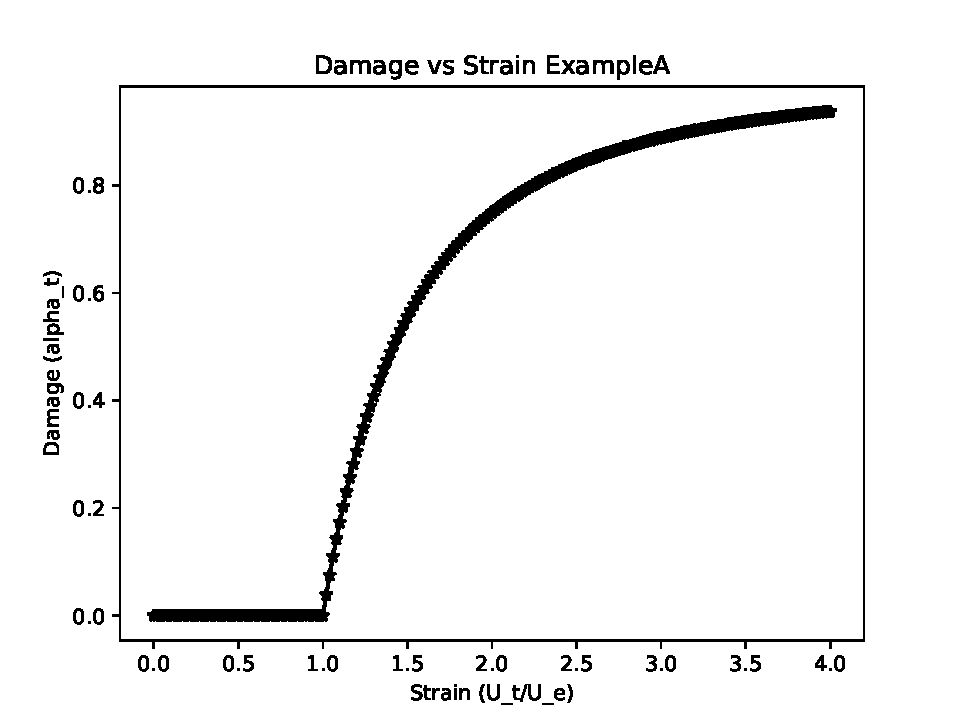
\includegraphics[width=\textwidth]{Images/A_damage_strain_dim.pdf}
    \end{subfigure}
    \quad %add desired spacing between images, e. g. ~, \quad, \qquad, \hfill etc. 
    \begin{subfigure}[b]{0.45\textwidth}
        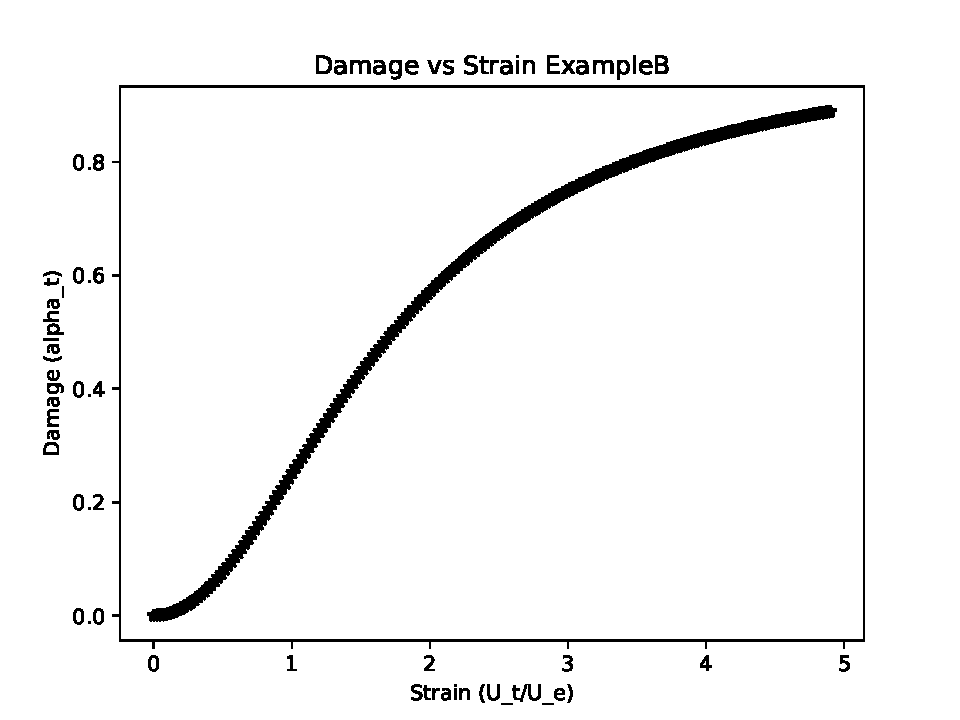
\includegraphics[width=\textwidth]{Images/B_damage_strain_dim.pdf}
    \end{subfigure}
    \caption{Damage vs strain property of the homogenous solution for A) example 1 and B) example 2}
\end{figure}
In example 1, after the elastic phase, the stress decreases asymptotically to 0. This feature illustrates stress softening. In example 2, there is no elastic phase. 
\begin{figure}[h]
    \centering
    \begin{subfigure}[b]{0.45\textwidth}
        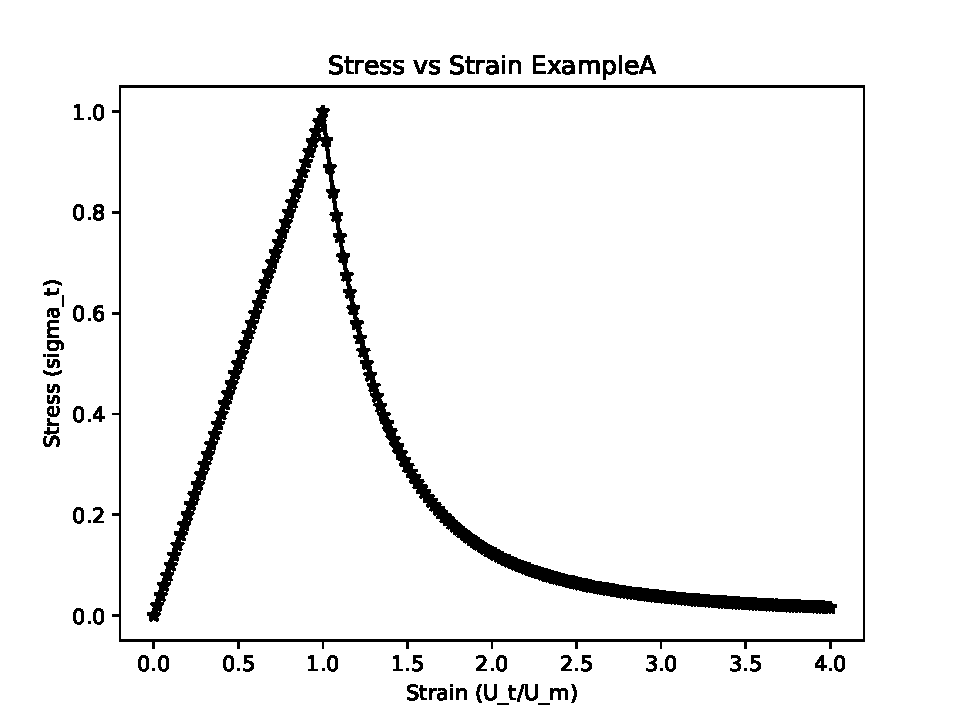
\includegraphics[width=\textwidth]{Images/A_stress_strain_dim.pdf}
    \end{subfigure}
    \quad %add desired spacing between images, e. g. ~, \quad, \qquad, \hfill etc. 
    \begin{subfigure}[b]{0.43\textwidth}
        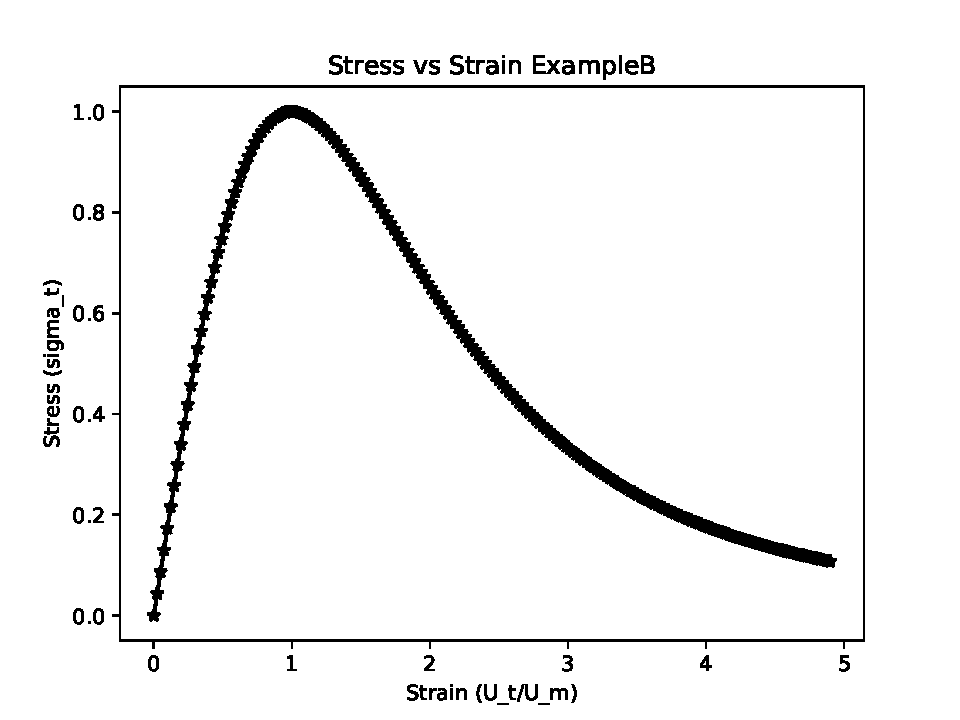
\includegraphics[width=\textwidth]{Images/B_stress_strain_dim.pdf}
    \end{subfigure}
    \caption{Stress vs. strain property of the homogenous solutions for A) example 1 and B) example 2}
\end{figure}

\subsection{Localized Solutions}
%====================================================================================
%====================================================================================

\subsubsection{Optimal Damage Profile}
%====================================================================================


\newpage 
\section{Appendix}
%====================================================================================
%====================================================================================
%====================================================================================
\subsection{Gateaux Derivative}\label{App:Gateaux}
%====================================================================================
%====================================================================================
The basic minimization problem is that we need to determine a suitable function $y = u(x) \in C^1 [a,b]$ that minimizes the objective functional (also known as the Lagrangian for the variational problem):
\begin{align}\label{objFunctional}
    J[u] = \int_a^b L(x,u, u') dx
\end{align}
In order to uniquely specific this function we must impose boundary conditions. These BCs depend on the problem. \\ \\
The gradient of the function, $\nabla J[u]$ of the functional will be defined by a directional derivative formula, where the inner product is defined with triangular brackets. 
\begin{align}\label{dirDerivative}
\langle \nabla J[u]; v\rangle = \frac{d}{d \epsilon} J[u+ \epsilon v] \bigg\rvert_{\epsilon = 0}   
\end{align}
Therefore, we can rewrite the objective functional as:
\begin{align*}
J[u] &= \int_a^b L(x,u, u') dx \\
J[u+\epsilon v] &= \int_a^b L(x,u+ \epsilon v, u' + \epsilon v') dx
\end{align*}
Then take the derivative with respect to $\epsilon$, and use the chain rule:
\begin{align*}
\frac{d}{d \epsilon} J[u+\epsilon v] &= \int_a^b \frac{d}{d \epsilon} L(x,u+ \epsilon v, u' + \epsilon v') dx \\
                                    &= \int_a^b \bigg[ \pdv{(u+ \epsilon v)}{\epsilon} \pdv{L}{(u + \epsilon v)} + \pdv{(u' + \epsilon v')}{\epsilon} \pdv{L}{(u' + \epsilon v')} \bigg] dx \\
                                    &= \int_a^b \bigg[ v \pdv{L}{(u + \epsilon v)} \big( x, u+ \epsilon v, u' + \epsilon v' \big) + v' \pdv{L}{(u'+\epsilon v')} \big( x, u+ \epsilon v, u' + \epsilon v' \big) \bigg] dx
\end{align*}
Next, set $\epsilon = 0$ as stated in Eq. \ref{dirDerivative}, and the result will be the first variation of the functional $J[u]$. 
\begin{align}\label{befIntParts}
\langle \nabla J[u]; v\rangle = \frac{d}{d \epsilon} J[u+ \epsilon v] \bigg\rvert_{\epsilon = 0} = \int_a^b \bigg[ v \pdv{L}{u} \big(x, u, u' \big) + v' \pdv{L}{u'} \big( x, u, u' \big) \bigg] dx 
\end{align}
The condition for a minimizer is known as the weak form of the variational principle
\begin{align}\label{wfVarPrin}
\langle \nabla J[u]; v\rangle &= 0
\end{align}
Eq. \ref{befIntParts} can be rephrased using integration by parts, which will yield a boundary term after the divergence theorem. In order to evaluate this problem, we will introduce Dirichlet boundary conditions 
\begin{align}\label{dirBC}
u(a) = \alpha \quad u(b) = \beta
\end{align}
Integration by parts formula, where we can say $r(x) = \pdv{L}{u'}$
\begin{align}\label{intByParts}
\begin{split}
(fg)' = f' g + f g' \rightarrow f' g &= (fg)' - f g' \\
                                v' r &= \pdv{}{x} \bigg(v r \bigg) - v \pdv{r}{x}  
\end{split}
\end{align}
Integrate over the domain, where boundary terms are zero
\begin{align*}
\int_a^b v' r dx &= \int_a^b \pdv{}{x} \bigg(v r \bigg) dx - \int_a^b v \pdv{r}{x} dx \\
                 &= v r \big\rvert_a^b - \int_a^b v \pdv{r}{x} dx \\
                 &= v(b) r(b) - v(a) r(a) - \int_a^b v \pdv{r}{x} dx \\
\int_a^b v' r dx &= - \int_a^b v \pdv{r}{x} dx
\end{align*}
where we can now calculate $r'(x)$ where $r(x) = \pdv{L}{u'}$
\begin{align*}
\begin{split}
r(x) &= \pdv{L}{u'} (x, u, u') \\
r'(x) &= \frac{d}{dx} \bigg(  \pdv{L}{u'} (x, u, u') \bigg) \\
r'(x) &= \pdv[2]{L}{x}{p} (x, u, u') + u' \pdv[2]{L}{x}{p} (x, u, u') + u'' \pdv[2]{L}{x}{p} (x, u, u')
\end{split}
\end{align*}
Substitute into the result from integration by parts: 
\begin{align*}
\int_a^b v' r dx &= - \int_a^b v \pdv{r}{x} dx \\
\int_a^b v' \pdv{L}{u'} \big(x, u, u' \big) dx &= - v \bigg[ \int_a^b \pdv[2]{L}{x}{p} (x, u, u') dx + \int_a^b u' \pdv[2]{L}{x}{p} (x, u, u') dx + \int_a^b u'' \pdv[2]{L}{x}{p} (x, u, u') dx \bigg] 
\end{align*}
Substitute into the first variation of the functional (Eq. \ref{befIntParts})
\begin{align}\label{aftIntParts}
\begin{split}
\langle \nabla J[u]; v\rangle &= \int_a^b \bigg[ v \pdv{L}{u} \big(x, u, u' \big) + v' \pdv{L}{u'} \big( x, u, u' \big) \bigg] dx \\
\langle \nabla J[u]; v\rangle &= \int_a^b v \pdv{L}{u} \big(x, u, u' \big) dx - v \bigg[ \int_a^b \pdv[2]{L}{x}{p} \big(x, u, u' \big) dx + \int_a^b u' \pdv[2]{L}{x}{p} \big(x, u, u' \big) dx + \int_a^b u'' \pdv[2]{L}{x}{p} \big(x, u, u' \big) dx \bigg] \\
\langle \nabla J[u]; v\rangle &= v \bigg[ \int_a^b \pdv{L}{u} \big(x, u, u' \big) dx - \int_a^b \pdv[2]{L}{x}{p} \big(x, u, u' \big) dx - \int_a^b u' \pdv[2]{L}{x}{p} \big(x, u, u' \big) dx - \int_a^b u'' \pdv[2]{L}{x}{p} \big(x, u, u' \big) dx \bigg]
\end{split}
\end{align}
Since this holds for all variations v(x), we can observe that the critical equation is a 2nd order differential equation known as the Euler-Lagrange Equation
\begin{align}\label{eulerLagrange}
\begin{split}
\nabla J [u] &= \pdv{L}{u} \big(x, u, u' \big) - \pdv[2]{L}{x}{p} \big(x, u, u' \big) - u' \pdv[2]{L}{x}{p} \big(x, u, u' \big) - u'' \pdv[2]{L}{x}{p} \big(x, u, u' \big) = 0 \\
E(x, u, u', u'') &= \pdv{L}{u} \big(x, u, u' \big) - \pdv[2]{L}{x}{p} \big(x, u, u' \big) - u' \pdv[2]{L}{x}{p} \big(x, u, u' \big) - u'' \pdv[2]{L}{x}{p} \big(x, u, u' \big) = 0 
\end{split}
\end{align}
\end{document}